\chapter{Introducci�n}

En este cap�tulo se har� una breve exposici�n sobre el proyecto final de carrera.

un poco de bla bla bla bla bla

Empezaremos con una introducci�n a la tegnolog�a Flash.

\section{�Qu� son las memorias Flash?}

La memoria flash es una evoluci�n de la memoria EEPROM, permite la lectura y escritura de m�ltiples posiciones de memoria en la misma operaci�n. Gracias a ello, la tecnolog�a flash, permite velocidades de funcionamiento muy superiores a la tecnolog�a EEPROM, que s�lo permit�a actuar sobre una �nica celda de memoria en cada operaci�n de programaci�n.

Utiliza una tecnolog�a de almacenamiento que mediante impulsos el�ctricos es capaz de leer, escribir o borrar informaci�n. Estas memorias est�n basadas en transistores de puerta flotante colocados formando celdas. El elemento b�sico de funcionamiento de las memorias son los transistores MOS de puerta-flotante \cite{IntroductionFlash}.

Fujio Masuoka en 1984 invent� este tipo de memoria como evoluci�n de las EEPROM existentes por aquel entonces, mientras trabajaba en Toshiba. Intel intent� atribuirse la creaci�n de esta sin �xito, aunque si comercializ� la primera memoria flash de uso com�n en 1988 [2].

Se dividen en dos clases seg�n el tipo de puertas usado en su fabricaci�n:
\begin{itemize}
  \item NAND: dise�adas con unas celdas muy peque�as, que permiten tener un precio muy peque�o por bit de almacenamiento.
  \item NOR: t�picamente se han usado para almacenar el software que luego es ejecutado en los dispositivos port�tiles.
\end{itemize}
En la actualidad la diferencia entre los dos tipos es cada vez menor \cite{FlashMemoryWikipedia}.


Que mierda pasa con el lineado !!!

asdfa

adfa
ads
adf


\begin{figure}
	\centering
		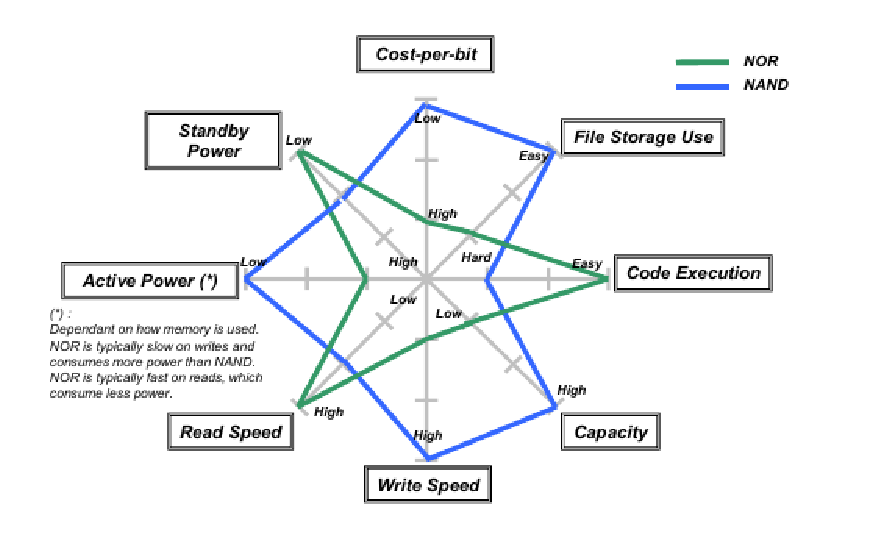
\includegraphics[width=0.60\textwidth,natwidth=610,natheight=642]{fig/comparacionNORNAN}
	\caption{\emph{Diferencia entre Flash NOR y NAND}}
\end{figure}
